\documentclass[twocolumn,11pt,letterpaper]{article}

% --- Packages ---
\usepackage[utf8]{inputenc}
\usepackage[T1]{fontenc}
\usepackage{amsmath}
\usepackage{amsfonts}
\usepackage{amssymb}
\usepackage{graphicx}
\usepackage{multirow}
\usepackage[pdf]{svg}
\usepackage{booktabs}
\usepackage{hyperref}
\usepackage[margin=1in]{geometry}
\usepackage{newtxtext,newtxmath}
\usepackage{microtype}
\usepackage{listings}
\lstset{basicstyle=\ttfamily,breaklines=true}

% --- Custom Abstract Formatting ---
\renewenvironment{abstract}
 {\small
  \begin{center}%
  \bfseries Abstract\vspace{-.5em}\vspace{0pt}%
  \end{center}%
  \list{}{%
    \setlength{\leftmargin}{0.5cm}%
    \setlength{\rightmargin}{\leftmargin}%
    \setlength{\parsep}{0pt}%
    \setlength{\parskip}{0pt}%
    \setlength{\itemsep}{0pt}%
  }%
  \item\relax}
 {\endlist}

% --- Hyperref Setup ---
\hypersetup{
    colorlinks=true,
    linkcolor=blue,
    filecolor=magenta,
    urlcolor=cyan,
    citecolor=green,
    pdftitle={Target and Stance Generation using Finetuned Llama},
    pdfsubject={Open-Target Stance Detection},
    pdfkeywords={Open-Target Stance Detection, Llama, Finetuning, LoRA, Stance Detection, Target Generation, PEFT, Semantic Evaluation},
}

% --- Title Block ---
\title{Target and Stance Generation using Finetuned Llama for Open-Target Stance Detection}

% --- Paragraph Formatting ---
\setlength{\parindent}{0pt}
\setlength{\parskip}{0.5em}

% --- Document Start ---
\begin{document}

\maketitle

% --- Abstract ---
\begin{abstract}
Open-Target Stance Detection (OTSD) requires identifying a target within a text and determining the expressed stance without prior knowledge of potential targets during inference, unlike traditional stance detection where targets are predefined. This study explores finetuning the Llama 3.1 8B model for OTSD using Parameter-Efficient Finetuning (PEFT) with Low-Rank Adaptation (LoRA) on a combined dataset from TSE and VAST resources. We evaluated the finetuned model against its base counterpart on three datasets: COVID-19 (specialized domain), EZStance Mixed (general-domain), and EZStance Noun Phrase (noun phrase targets). Semantic assessment by Gemini and DeepSeek-671B, averaged for robustness, and BERTweet-based similarity confirmed the finetuned model's superior performance, particularly on COVID-19, achieving 66.30\% stance accuracy and 52.47\% target accuracy (vs. 45.28\% and 25.39\% for the base model). EZStance Mixed showed moderate gains, while EZStance Noun Phrase exhibited significant target accuracy improvement but a slight stance accuracy decline, underscoring domain-specific challenges. These results highlight the efficacy of finetuning for OTSD.
\end{abstract}

% --- Keywords ---
\noindent\textbf{Keywords:} Open-Target Stance Detection, Llama, Finetuning, LoRA, Stance Detection, Target Generation, Parameter-Efficient Finetuning, Semantic Evaluation.

% --- Sections ---

\section{Introduction}
\label{sec:introduction}

Stance Detection (SD) is a fundamental task in natural language processing, focusing on determining the viewpoint (e.g., favor, against, neutral) expressed in a text towards a given entity or topic, known as the target \cite{akash2024}. Many real-world applications, such as social media analysis, opinion polling, and argument mining, benefit from accurate stance detection. However, a significant limitation of many existing SD approaches is the requirement that the target of the stance be provided beforehand. This assumption does not hold in many practical scenarios where the target itself needs to be identified from the text.

This leads to the more complex and realistic task of Open-Target Stance Detection (OTSD), where the model must first identify the relevant target(s) within the text and then determine the stance towards that identified target \cite{akash2024}. The OTSD task presents challenges in both target generation (TG) and subsequent stance classification, especially when targets are not explicitly mentioned. While Zero-Shot Stance Detection (ZSSD) methods have emerged to handle targets unseen during training \cite{vast}, they typically still require the target to be provided during inference. Even recent approaches like Target-Stance Extraction (TSE) , which generate targets, often rely on mapping these generated targets to a predefined list, limiting their truly "open" nature.

Recent advancements in Large Language Models (LLMs) have shown promise in various zero-shot and few-shot learning scenarios. Their ability to understand context and generate text makes them potential candidates for tackling the complexities of OTSD. Initial work by Akash et al. \cite{akash2024} explored the zero-shot capabilities of various LLMs, including Llama, for OTSD, highlighting their potential but also the challenges, particularly with non-explicit targets.

This paper investigates the effectiveness of \textit{finetuning} an LLM for the OTSD task. Specifically, we focus on the Llama 3.1 8B architecture \cite{llama3.1} and employ Parameter-Efficient Finetuning (PEFT) using Low-Rank Adaptation (LoRA) \cite{lora}. We train the model on a combined dataset derived from existing stance detection resources (TSE and VAST datasets, as used in \cite{akash2024}) to simultaneously generate the target and predict the stance in a specific format. We evaluate the performance of the finetuned model against its base zero-shot counterpart on three distinct test datasets (COVID-19, EZStance Mixed, EZStance Noun Phrase) using semantic evaluation performed by state-of-the-art LLMs (Gemini and DeepSeek-671B). Our contribution lies in demonstrating the impact of task-specific finetuning via LoRA on the Llama model's ability to address the joint target generation and stance detection challenges inherent in OTSD, with particularly strong improvements in specialized domains like COVID-19 and more moderate gains in general-domain datasets.

\section{Literature Review}
\label{sec:literature}

Research in Stance Detection (SD) has evolved significantly. Early work focused on supervised classification tasks where both the text and the target were provided, often using feature engineering and traditional machine learning models, later transitioning to deep learning approaches like LSTMs and CNNs \cite{vast}.

Recognizing the impracticality of gathering labeled data for every conceivable target, Zero-Shot Stance Detection (ZSSD) emerged. ZSSD aims to predict stances towards targets unseen during training. Various techniques have been explored, including contrastive learning, generative approaches, prompt-based learning with LLMs, and methods incorporating external knowledge \cite{vast}. A prominent line of work, TSE , generates targets but subsequently maps them to a known target list, facilitating evaluation but deviating from a truly open-target scenario.

The specific challenge of Open-Target Stance Detection (OTSD), where the target is neither provided nor drawn from a predefined inference-time list, was formally introduced and benchmarked by Akash et al. \cite{akash2024}. Their work evaluated the zero-shot performance of several state-of-the-art LLMs (GPT-3.5, GPT-4o, Mistral) on OTSD, establishing baseline capabilities and highlighting the difficulty posed by implicitly mentioned targets. They demonstrated that while LLMs outperform prior methods in target generation quality, significant challenges remain.

Contemporaneously, the capabilities of Large Language Models (LLMs) like Llama \cite{llama3.1}, GPT, and Mistral have rapidly advanced. Their success in diverse generative and instruction-following tasks suggests their potential for the joint generation requirement of OTSD.

However, fully finetuning such large models is computationally expensive. Parameter-Efficient Finetuning (PEFT) methods have been developed to mitigate this. Among these, Low-Rank Adaptation (LoRA) \cite{lora} is a popular technique that introduces trainable low-rank matrices into the existing layers of an LLM, allowing adaptation with significantly fewer trainable parameters compared to full finetuning.

This work builds directly upon the OTSD task defined by Akash et al. \cite{akash2024}. Instead of evaluating zero-shot performance, we investigate the impact of applying PEFT (specifically LoRA) to finetune a Llama 3.1 8B model explicitly for the combined target generation and stance classification task inherent in OTSD.

\section{Methodology}
\label{sec:methodology}

Our approach to Open-Target Stance Detection (OTSD) involves adapting a pretrained Large Language Model to jointly generate the stance target and classify the stance expressed towards it within a given input text.

\subsection{Problem Definition}
\label{sec:problem_definition}

Let the training dataset be represented as $D = \{(x_i, t_i, y_i)\}_{i=1}^{N}$, where $x_i$ denotes the input text, $t_i$ is the corresponding ground truth target, and $y_i$ is the ground truth stance label (e.g., "FAVOR", "AGAINST", "NONE"). The test dataset is represented similarly as $D' = \{(x'_j, t'_j, y'_j)\}_{j=1}^{M}$, where $x'_j$ represents an input text potentially containing novel targets not seen in $D$.

The core objective in Open-Target Stance Detection (OTSD) is to train a model $M$ that, given an input text $x'$, generates an output sequence $O$ encompassing both a predicted target $\hat{t'}$ and a predicted stance $\hat{y'}$.
Formally:
\[ O = M(x') \]

The generated output sequence $O$ must be parsable to extract the predicted target $\hat{t'}$ and stance $\hat{y'}$. In our implementation, the model is trained using supervised finetuning on $D$ to produce outputs formatted precisely according to a predefined template:

\begin{lstlisting}[basicstyle=\small\ttfamily,columns=flexible,breaklines=true,breakatwhitespace=true,frame=single]
Below is an instruction that describes a task, paired with an input that provides further context. Write a response that appropriately completes the request.

### Instruction:
Analyze the stance and identify the target in the following text.

### Input:
[Input Text]

### Response:
Target: [Target], Stance: [Stance]<|end_of_text|>
\end{lstlisting}

During inference, the \texttt{[Target]} and \texttt{[Stance]} parts are left empty for the model to generate. The goal is to train $M$ such that for unseen inputs $x'$ from the test distribution $D'$, the generated $\hat{t'}$ closely approximates the ground truth target $t'$ and the predicted stance $\hat{y'}$ matches the ground truth stance $y'$.

\subsection{System Overview}
\label{sec:system_overview}

Figure \ref{fig:system_diagram} presents the high-level architecture of our OTSD system. The pipeline consists of three main components:

\begin{itemize}
    \item \textbf{Input Processing}: The system accepts raw text input from various sources such as social media posts and news comments.
    \item \textbf{Model Processing}: A finetuned Llama 3.1 8B model with LoRA adaptations processes the input, optimized using 4-bit quantization and the Unsloth library.
    \item \textbf{Structured Output}: The model generates structured data containing the identified target and corresponding stance.
\end{itemize}

\begin{figure*}[t]
\centering
\includesvg[width=0.95\textwidth]{figures/system_diagram}
\caption{High-Level OTSD System Diagram showing the complete pipeline from raw text input to structured stance and target output. The system utilizes a finetuned Llama 3.1 8B model with LoRA adaptations, optimized using 4-bit quantization and the Unsloth library.}
\label{fig:system_diagram}
\end{figure*}

\begin{figure*}[t]
\centering
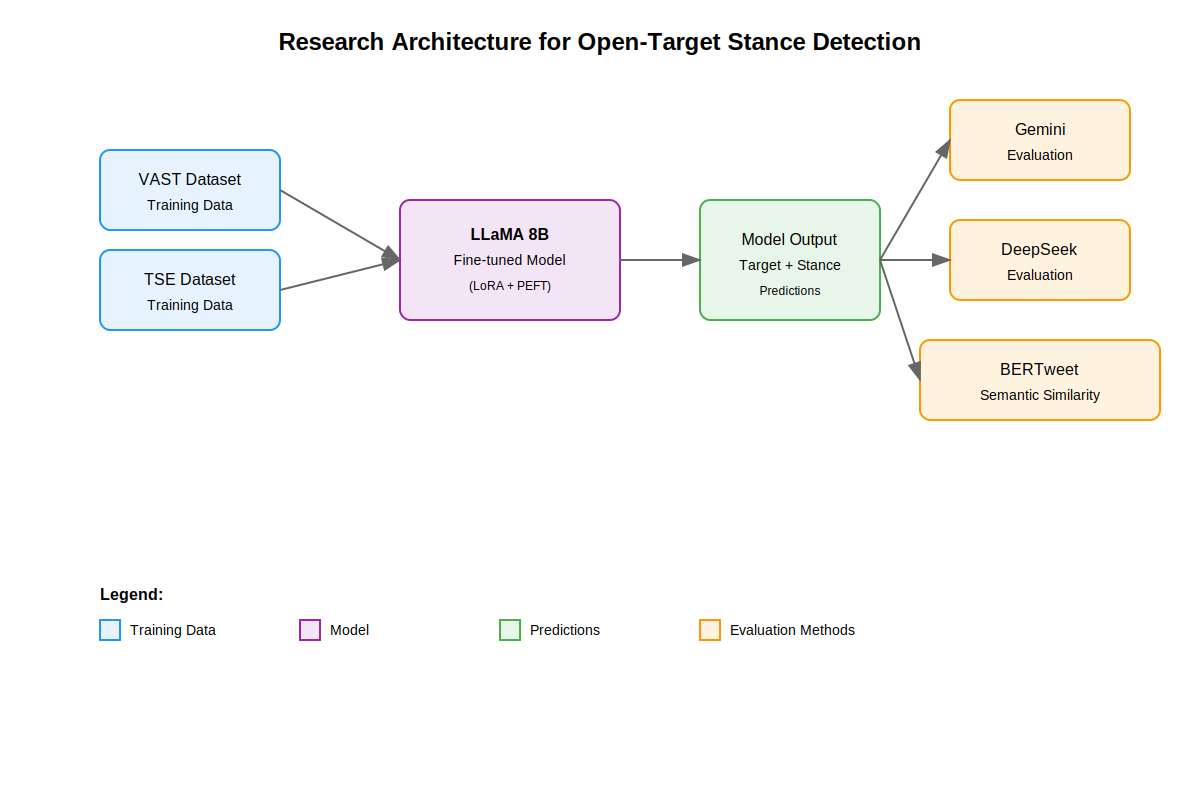
\includegraphics[width=0.95\textwidth]{figures/research_architecture.pdf}
\caption{Detailed Research Architecture showing the complete pipeline from training data through model finetuning to evaluation. The system combines VAST and TSE datasets for training, processes through a finetuned Llama 3.1 8B model, and evaluates outputs using multiple methods including Gemini, DeepSeek, and BERTweet for semantic similarity assessment.}
\label{fig:research_arch}
\end{figure*}

\subsection{Model Architecture}
\label{sec:model_arch}

Our approach adapts a Large Language Model (LLM) for the specific demands of Open-Target Stance Detection (OTSD). While the base model possesses extensive pre-trained capabilities, achieving optimal performance on this nuanced task necessitates task-specific adaptation. Fully finetuning large models like Llama 3.1 8B demands substantial computational resources (GPU memory and time) often unavailable in typical research settings. To overcome this limitation, we employed \textbf{Parameter-Efficient Finetuning (PEFT)}, a family of techniques designed to adapt large pretrained models by modifying only a small fraction of their parameters.

Specifically, we adopted \textbf{Low-Rank Adaptation (LoRA)} \cite{lora}. LoRA operates on the principle that the change in weights required to adapt a pretrained model to a new task often has a low intrinsic rank. Instead of learning the full change $\Delta W$ for a weight matrix $W$, LoRA learns its low-rank decomposition $\Delta W = BA$, where $B \in \mathbb{R}^{d \times r}$ and $A \in \mathbb{R}^{r \times k}$ are significantly smaller matrices (the "LoRA adapters") with rank $r \ll \min(d, k)$. During finetuning, the original pretrained weights $W$ are kept frozen, and only the parameters within the newly introduced matrices $A$ and $B$ are updated via gradient descent. The effective weight matrix during forward passes becomes $W + BA$, as illustrated in Figure \ref{fig:llama_lora_arch}. This approach dramatically reduces the number of trainable parameters; in our setup, only approximately 0.52\% of the total model parameters were trained, making finetuning feasible.

\begin{figure}[htbp]
\centering
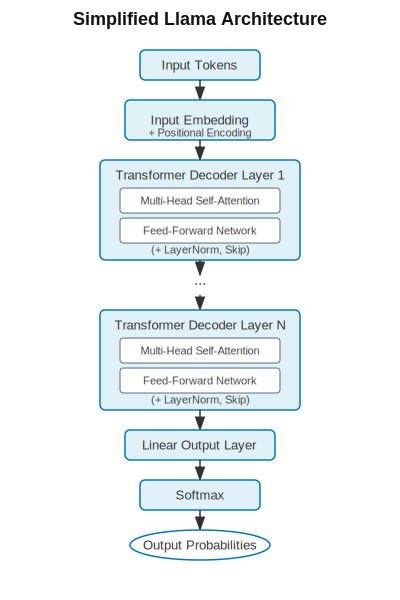
\includegraphics[width=1\columnwidth]{figures/llama_arc.pdf}
\caption{Detailed Llama 3.1 8B Architecture with LoRA adapters applied for OTSD finetuning. Base model weights (including embeddings and output layer) remain frozen, while LoRA modules are inserted into attention and feed-forward layers and are the only components trained.}
\label{fig:llama_lora_arch}
\end{figure}

The specific configuration of LoRA in our experiments, guided by the implementation in the accompanying notebook and common practices for effective adaptation, included:
\begin{itemize}
    \item \textbf{Rank ($r$):} Set to \textbf{16}. This determines the inner dimension of the LoRA matrices $A$ and $B$, controlling the capacity of the adaptation.
    \item \textbf{LoRA Alpha ($\alpha$):} Set to \textbf{16}. This acts as a scaling factor for the LoRA update. The effective update applied to the forward pass is $(\alpha / r) \times BA$. Setting $\alpha = r$ is a common initialization strategy.
    \item \textbf{Targeted Modules:} LoRA adapters were strategically injected into specific layers crucial for language processing within the Llama architecture. These included the query (\texttt{q\_proj}), key (\texttt{k\_proj}), value (\texttt{v\_proj}), and output (\texttt{o\_proj}) projection layers within the multi-head self-attention mechanism, as well as the gate (\texttt{gate\_proj}), up (\texttt{up\_proj}), and down (\texttt{down\_proj}) projection layers within the feed-forward network blocks. These modules were selected as they are critical for adapting the attention and feed-forward components of the transformer architecture.
    \item \textbf{LoRA Dropout:} Set to 0, disabling dropout within the LoRA layers for optimized performance as suggested by Unsloth.
    \item \textbf{Bias:} Set to \texttt{"none"}, indicating that bias terms within the LoRA adapters were not trained.
\end{itemize}

The foundation for this adaptation is the \textbf{Llama 3.1 8B} model \cite{llama3.1}, a highly capable LLM developed by Meta. As a member of the Llama family, Llama 3.1 8B represents the cutting edge in open foundation models, pretrained on trillions of tokens from a diverse range of publicly available sources. Architecturally, it follows the standard \textbf{transformer-based, decoder-only} paradigm. This means the model processes input sequences and autoregressively generates output tokens one after another, conditioning each new token on the preceding sequence. This inherent generative capability makes it well-suited for tasks requiring text production, such as the joint target and stance generation needed for OTSD. The 8B parameter variant strikes a balance between strong performance and manageable computational requirements. For our experiments, we specifically utilized the \texttt{unsloth/Meta-Llama-3.1-8B}\footnote{Available at \url{https://huggingface.co/unsloth/Meta-Llama-3.1-8B}} version available on Hugging Face.

To facilitate the finetuning process on resource-constrained hardware (specifically, an NVIDIA T4 GPU with approx. 15GB VRAM as used in the notebook environment), we leveraged the \textbf{Unsloth library} \cite{unsloth}. Unsloth provides optimized implementations for faster training and reduced memory usage. Key techniques enabled by Unsloth in our setup were:
\begin{itemize}
    \item \textbf{4-bit Quantization:} The base Llama 3.1 8B model weights were loaded in 4-bit precision (\texttt{load\_in\_4bit = True}) using bitsandbytes . This technique significantly compresses the model size, reducing the GPU memory required to load the model.
    \item \textbf{Gradient Checkpointing:} We utilized Unsloth's optimized implementation of gradient checkpointing (\texttt{use\_gradient\_checkpointing = "unsloth"}). This technique avoids storing all intermediate activations during the forward pass, instead recomputing them during the backward pass, drastically reducing memory usage at the cost of increased computation time, enabling training with a sequence length of 2048 tokens.
\end{itemize}

The resulting model, incorporating the frozen Llama 3.1 8B base weights and the trained LoRA adapters, constitutes our finetuned OTSD model ($M_{\text{finetuned}}$). This architecture is compared against the performance of the base 4-bit quantized Llama 3.1 8B model ($M_{\text{base}}$) used directly for the task without LoRA adapters or finetuning.

\subsection{Datasets}
\label{sec:dataset}

Our work utilizes several datasets for finetuning and evaluation, covering diverse domains and stance targets:

\subsubsection{Finetuning Dataset}
For finetuning the Llama 3.1 8B model, we constructed a combined dataset by merging resources from established stance detection benchmarks:
\begin{itemize}
    \item \textbf{TSE Dataset} \cite{tse_data}: Focuses on Target-Stance Extraction, providing examples with explicitly mentioned targets and stances. It includes a variety of social media texts with labeled targets and stances.
    \item \textbf{VAST Dataset} \cite{vast_data}: Offers a variety of topics and stances, contributing to the diversity of the training data. It covers multiple domains, enhancing the model's ability to generalize.
\end{itemize}
This combined dataset, comprising 6,480 examples (as per the notebook logs), was used exclusively for the PEFT process. Each entry contained the input text, the ground truth target, and the ground truth stance (FAVOR, AGAINST, or NONE), formatted into the instruction-following template described in Section \ref{sec:problem_definition}.

Importantly, the training and test datasets contain no common texts, underscoring the open stance target detection nature of this study.

Table \ref{tab:training_samples} presents representative examples from our training dataset, showcasing the diversity of topics and stance expressions.

\begin{table*}[!htbp]
\centering
\caption{Sample Training Data Points}
\label{tab:training_samples}
\begin{tabular}{|p{0.55\textwidth}|p{0.25\textwidth}|p{0.1\textwidth}|}
\hline
\textbf{Text} & \textbf{Target} & \textbf{Stance} \\
\hline
Necessity is the mother of all invention. Never bet against human ingenuity, especially when survival is on the line. The technology we need to move beyond fossil fuels exist today - wind, solar, efficiency improvements like LED lighting, and especially nuclear power. & technology & AGAINST \\
\hline
Other ways to heal: when you can't tell your \#MeToo story. The technology we need to move beyond fossil fuels exist today. & metoo movement & AGAINST \\
\hline
COMCAST willing to outbid Disney for Fox... could the deal between Disney and Fox be over? & merger of disney and fox & AGAINST \\
\hline
\end{tabular}
\end{table*}

\subsubsection{Evaluation Datasets}
To rigorously evaluate the performance and generalization capabilities of both the base and finetuned models, we employed three distinct test datasets, separate from the finetuning data. Table \ref{tab:test_samples} presents representative examples from each test dataset.

\begin{table*}[!htbp]
\centering
\caption{Sample Test Data Points from Different Evaluation Datasets}
\label{tab:test_samples}
\begin{tabular}{|p{0.6\textwidth}|p{0.2\textwidth}|p{0.1\textwidth}|}
\hline
\textbf{Text} & \textbf{Target} & \textbf{Stance} \\
\hline
\multicolumn{3}{|c|}{COVID-19 Dataset} \\
\hline
Maybe if people want to walk around without masks on they can organize into fenced-off private mask nudist colonies, keep their idiotic sense of liberty, and the rest of us can live in a society. \#WearAMask & face masks & FAVOR \\
\hline
\multicolumn{3}{|c|}{EZStance Mixed Dataset} \\
\hline
WhiteHouse has appealed a Trump-appointed judge's obstruction of CDCgov's transportation mask mandate, but without an emergency stay, millions of lives remain in danger as we work our way through the courts. & Trump-appointed judge & AGAINST \\
\hline
\multicolumn{3}{|c|}{EZStance Noun Phrase Dataset} \\
\hline
Fgs stop calling Cummings a mad genius. He's just mad. The higher echelons of the civil service are as hidebound by private education as the Tory party, law and the BBC. & Cummings & AGAINST \\
\hline
\end{tabular}
\end{table*}

\begin{itemize}
    \item \textbf{COVID-19}: A dataset focused specifically on stances related to the COVID-19 pandemic, representing a specialized domain with domain-specific terminology and sentiment.
    \item \textbf{EZStance Mixed} \cite{akash2024}: A general-domain dataset containing a mix of topics and targets, testing the model's ability to handle diverse inputs.
    \item \textbf{EZStance Noun Phrase} \cite{akash2024}: Focuses on noun phrases as targets, presenting a unique linguistic challenge that may affect stance classification due to the abstract or implicit nature of targets.
\end{itemize}
These datasets served as the held-out test sets for evaluating both the base and finetuned models using the semantic evaluation methodology outlined in Section \ref{sec:results}.

\subsection{Finetuning Details}
\label{sec:finetuning}

The finetuning process was carried out using the Supervised Finetuning Trainer (\texttt{SFTTrainer})\footnote{Available at \url{https://huggingface.co/docs/trl/index}} from the Hugging Face TRL library, integrated with the Unsloth optimizations. The training objective was standard causal language modeling loss, where the model learns to predict the next token in the sequence, specifically trained to generate the \texttt{Target: ..., Stance: ...} response based on the provided instruction and input text.

\subsection{Training Configuration}
The model was trained with a maximum sequence length of 2048 tokens. We used a per-device training batch size of 2 and gradient accumulation steps of 4, resulting in an effective batch size of 8. The learning rate was set to $2 \times 10^{-4}$ with a linear decay scheduler and 5 warmup steps. Optimization was performed using the AdamW 8-bit optimizer. Training was conducted for a maximum of 60 steps. Floating point precision was set to BF16 if supported, otherwise FP16 was used. A seed of 3407 was used for reproducibility.

\begin{figure}[htbp]
\centering
\includesvg[width=\columnwidth]{figures/training_loss_plot.svg}
\caption{Training loss curve for the Llama 3.1 8B model finetuned for OTSD over 60 steps.}
\label{fig:training_loss}
\end{figure}

\subsection{Evaluation Metrics}
\label{sec:eval_metrics}
To evaluate model performance, we employed several metrics focusing on both target generation and stance classification:

\textbf{Semantic Evaluation (DeepSeek \& Gemini):} The primary evaluation involved semantic assessment by state-of-the-art LLMs, DeepSeek-671B and Gemini. This process involved providing the original input text, the ground truth target, the ground truth stance, the model-predicted target, and the model-predicted stance to both evaluators. These models then assessed the semantic correctness and similarity of the predicted target and stance compared to the ground truth, assigning a score represented as a percentage accuracy (shown in Table \ref{tab:combined_results}). The "Average" columns in Table \ref{tab:combined_results} represent the arithmetic mean of the scores obtained from DeepSeek and Gemini for stance and target accuracy, respectively, providing a balanced measure of performance.

The percentage accuracy for each metric is computed as:
\[
\text{Accuracy} = \frac{1}{N} \sum_{i=1}^{N} \text{score}_i \times 100
\]
where $\text{score}_i$ is the semantic evaluation score (either binary or continuous) for the $i$-th test example, and $N$ is the total number of test examples.

For each example $i$:
\[
\text{score}_i = \text{LLM}_\text{sem}(y_i, \hat{y}_i, t_i, \hat{t}_i)
\]
where $\text{LLM}_\text{sem}$ denotes the percentage score assigned by the LLM evaluator based on the semantic similarity between the ground truth stance $y_i$, predicted stance $\hat{y}_i$, ground truth target $t_i$, and predicted target $\hat{t}_i$.

\textbf{Target Semantic Similarity (BERTweet Score - BTSD):} We employed BERTweet \cite{bertweet} specifically for semantic similarity assessment of predicted targets against the ground truth target. BERTweet provides a specialized evaluation metric suited for measuring semantic similarity in social media text. It is important to note that while BERTweet provides valuable sentence-level semantic insights, its performance might be less optimal for fine-grained word-level semantic analysis, as it was primarily developed for evaluating sentence similarity. The BERTweet Similarity score (referred to as BTSD in Table \ref{tab:comparison}) is reported in Table \ref{tab:bertweet_results}.

The BTSD score is computed as:
\[
\text{BTSD} = \frac{1}{N} \sum_{i=1}^{N} \text{BERTweetSim}_i \times 100
\]
where $\text{BERTweetSim}_i$ is the BERTweet similarity score for the $i$-th test example.

For each example $i$:
\[
\text{BERTweetSim}_i = \text{BERTweetSim}(t_i, \hat{t}_i)
\]
where $\text{BERTweetSim}$ denotes the similarity score (between 0 and 100) computed by BERTweet between the ground truth target $t_i$ and the predicted target $\hat{t}_i$.

\textbf{Stance Classification Accuracy (SC \%):} For direct comparison with previous work as presented in Table \ref{tab:comparison}, we use Stance Classification accuracy (SC \%). This metric reflects the percentage of correctly predicted stance labels (FAVOR, AGAINST, NONE).

The SC percentage is computed as:
\[
\text{SC} = \frac{1}{N} \sum_{i=1}^{N} \mathbb{I}(\hat{y}_i = y_i) \times 100
\]
where $\mathbb{I}(\hat{y}_i = y_i)$ is 1 if the predicted stance $\hat{y}_i$ matches the ground truth $y_i$, and 0 otherwise.

\section{Results and Discussion}
\label{sec:results}

We evaluated our models on three distinct datasets to assess their generalization capabilities and performance across different domains. The results are presented for both the base Llama model ($M_{\text{base}}$) and the finetuned model ($M_{\text{finetuned}}$), using the evaluation metrics described in Section \ref{sec:eval_metrics}. 
Table \ref{tab:combined_results} presents the comprehensive semantic evaluation results across all datasets.

\begin{table*}[!htbp]
\centering
\caption{Comprehensive Semantic Evaluation Results (\%): Accuracy is based on the semantic correctness and similarity of the predicted target and stance compared to the ground truth, assigning a score represented as a percentage.}
\label{tab:combined_results}
\begin{tabular}{@{}llcccccc@{}}
\toprule
\textbf{Dataset} & \textbf{Model} & \multicolumn{2}{c}{\textbf{DeepSeek}} & \multicolumn{2}{c}{\textbf{Gemini}} & \multicolumn{2}{c}{\textbf{Average}} \\
\cmidrule(lr){3-4} \cmidrule(lr){5-6} \cmidrule(lr){7-8}
& & Stance & Target & Stance & Target & Stance & Target \\
\midrule
\multirow{2}{*}{COVID-19} 
& Base & 47.22 & 25.57 & 43.33 & 25.21 & 45.28 & 25.39 \\
& Finetuned & \textbf{71.43} & 42.24 & 61.17 & \textbf{62.69} & \textbf{66.30} & \textbf{52.47} \\
\midrule
\multirow{2}{*}{EZStance Mixed} 
& Base & 43.78 & 26.94 & 44.22 & 26.03 & 44.00 & 26.49 \\
& Finetuned & \textbf{50.00} & \textbf{34.26} & 48.48 & 33.31 & \textbf{49.24} & \textbf{33.79} \\
\midrule
\multirow{2}{*}{EZStance Noun Phrase} 
& Base & \textbf{48.99} & 27.09 & 46.67 & 25.70 & \textbf{47.83} & 26.40 \\
& Finetuned & 47.13 & \textbf{35.29} & 47.11 & 34.07 & 47.12 & \textbf{34.68} \\
\bottomrule
\end{tabular}
\end{table*}

\begin{table*}[!htbp]
\centering
\caption{BERTweet Evaluation: Comparing Target Semantic Similarity (BERTweet Score) and Stance Classification Performance (Macro F1 Score) for Base and Finetuned Models}
\label{tab:bertweet_results}
\begin{tabular}{@{}llcc@{}}
\toprule
\textbf{Dataset} & \textbf{Model} & \textbf{BERTweet Similarity} & \textbf{Macro F1} \\
\midrule
\multirow{2}{*}{COVID-19} 
& Base & 0.7363 & 0.2660 \\
& Finetuned & \textbf{0.7832} & \textbf{0.2947} \\
\midrule
\multirow{2}{*}{EZStance Mixed} 
& Base & 0.7392 & 0.3624 \\
& Finetuned & \textbf{0.7779} & \textbf{0.3964} \\
\midrule
\multirow{2}{*}{EZStance Noun Phrase} 
& Base & 0.7390 & 0.3533 \\
& Finetuned & \textbf{0.7871} & \textbf{0.3907} \\
\bottomrule
\end{tabular}
\end{table*}

\subsection{Comparison with Previous Work}
\begin{table*}[!htbp]
\centering
\caption{Comparison of Finetuned Llama 3.1 8B with Base Model and Previous Work (Akash et al.) on EZStance Datasets. Metrics shown are Target Generation (BTSD Score) and Stance Detection Accuracy (SC \%).}
\label{tab:comparison}
\begin{tabular}{|p{0.24\textwidth}|p{0.15\textwidth}|p{0.2\textwidth}|p{0.2\textwidth}|}
\hline
\textbf{Model} & \textbf{Dataset} & \textbf{Target Generation (BTSD)} & \textbf{Stance Detection (SC)} \\
\hline
\multirow{2}{*}{Finetuned Llama 3.1 8B} 
& EZStance Mixed & 77.79 & 49.24 \\
\cline{2-4}
& EZStance NP & 78.71 & 47.12 \\
\hline
\multirow{2}{*}{Base Llama 3.1 8B} 
& EZStance Mixed & 73.92 & 44.00 \\
\cline{2-4}
& EZStance NP & 73.90 & 47.83 \\
\hline
\multirow{2}{*}{GPT-4o~\cite{akash2024}} 
& EZStance Mixed & 50.69 & 46.22 \\
\cline{2-4}
& EZStance NP & 50.69 & 46.22 \\
\hline
\multirow{2}{*}{Mistral~\cite{akash2024}} 
& EZStance Mixed & 50.17 & 48.72 \\
\cline{2-4}
& EZStance NP & 50.17 & 48.72 \\
\hline
\end{tabular}
\end{table*}

The comparison reveals several key insights:
\begin{itemize}
    \item For EZStance Mixed, our model achieves better overall performance compared to previous zero-shot approaches
    \item In the EZStance Noun Phrase dataset, while target identification improved significantly, stance detection showed mixed results compared to previous work.
\end{itemize}

\subsection{Analysis of Results}
Several key observations emerge from these results:

\begin{itemize}
    \item \textbf{COVID-19 Dataset Performance}: The most substantial improvements were observed in the COVID-19 dataset, where the finetuned model achieved: 
    
    An average stance accuracy increase of 21.02 percentage points (from 45.28\% to 66.30\%) was observed, along with an average target accuracy increase of 27.08 percentage points (from 25.39\% to 52.47\%).
    
    \item \textbf{EZStance Mixed Dataset}: Significant improvements were seen across all metrics: 
    
    Average stance accuracy improved by 5.24 percentage points, and average target accuracy improved by 7.30 percentage points. BERTweet semantic similarity increased from 0.7392 to 0.7779, and the Macro F1 score improved from 0.3624 to 0.3964.
    
    \item \textbf{EZStance Noun Phrase Dataset}: Consistent improvements across all metrics: 
    
    Average target accuracy increased by 8.28 percentage points. BERTweet semantic similarity improved from 0.7390 to 0.7871, and the Macro F1 score increased from 0.3533 to 0.3907.
    
    \item \textbf{Evaluator Consistency}: The averaged results from DeepSeek and Gemini demonstrate consistent trends, though with some variations: 
    
    DeepSeek typically showed higher stance accuracy scores, while Gemini often provided higher target accuracy scores. The variation may stem from differences in their training data or architectural biases, with DeepSeek potentially better tuned for stance classification and Gemini for semantic target matching. The averaged metrics provide a balanced view of model performance.
\end{itemize}

These results demonstrate that our finetuning approach is particularly effective for specialized domains like COVID-19, while still providing meaningful improvements across more general datasets. The consistent improvement in target identification across all datasets validates the effectiveness of our approach for the core challenge of target extraction in OTSD. The averaged metrics from both evaluators provide a robust measure of performance, helping to mitigate potential biases from any single evaluation model.

\section{Error Analysis}

To better understand the types of errors made by the finetuned model, we present the confusion matrix in Figure~\ref{fig:confusion_matrix}. This matrix summarizes the model's stance predictions (FAVOR, AGAINST, NONE) against the ground truth labels across the test set. The diagonal elements represent correct predictions, while off-diagonal elements indicate misclassifications. Notably, the model achieves high accuracy for the FAVOR and AGAINST classes, but some confusion remains, particularly between NONE and the other stances. This suggests that distinguishing neutral or ambiguous cases remains a challenge for the model, possibly due to the inherent subjectivity and context-dependence of stance in open-domain settings.

% --- Error Analysis Table: Segregated by Performance ---

\begin{table*}[!htbp]
    \centering
    \caption{Sample Error Analysis: Segregated Examples of Model Successes and Failures}
    \label{tab:error_analysis_examples}
    \begin{minipage}{0.98\textwidth}
    \centering
    \textbf{(a) Performed Well: Representative Examples}
    \vspace{0.5em}
    \begin{tabular}{|p{0.40\textwidth}|p{0.13\textwidth}|p{0.13\textwidth}|p{0.13\textwidth}|p{0.13\textwidth}|}
    \hline
    \textbf{Original Text} & \textbf{Ground Truth Target} & \textbf{Ground Truth Stance} & \textbf{Predicted Target} & \textbf{Predicted Stance} \\
    \hline
    We wore our masks to ensure the safety of staff and customers & face masks & FAVOR & face masks & FAVOR \\
    \hline
    Cummings is just mad. The higher echelons of the civil service are as hidebound by private education as the Tory party, law and the BBC. & Cummings & AGAINST & Cummings & AGAINST \\
    \hline
    Central Bank of Kenya Pension Towers, a 27-storey skyscraper in Nairobi is receiving special attention from China due to its world class architectural design. It was by Kenyan Architects. It has solar panels, which enables it to supply its own clean energy during the day. & Central Bank of Kenya Pension Towers & FAVOR & Central Bank of Kenya Pension Towers & FAVOR \\
    \hline
    U.S State Department officials met with the Phoenix Mercury today to discuss steps to safely get Brittney Griner out of Russia. Democratic Congressman Greg Stanton was in attendance and said he's leading a bipartisan solution in Congress calling for Griner's immediate release. & Brittney Griner & FAVOR & Brittney Griner & FAVOR \\
    \hline
    "Fgs stop calling Cummings a mad genius. He's just mad." & Cummings & AGAINST & Cummings & AGAINST \\
    \hline
    \end{tabular}
    \vspace{1em}
    \textbf{(b) Did Not Perform Well: Representative Examples}
    \vspace{0.5em}
    \begin{tabular}{|p{0.40\textwidth}|p{0.13\textwidth}|p{0.13\textwidth}|p{0.13\textwidth}|p{0.13\textwidth}|}
    \hline
    \textbf{Original Text} & \textbf{Ground Truth Target} & \textbf{Ground Truth Stance} & \textbf{Predicted Target} & \textbf{Predicted Stance} \\
    \hline
    Thank goodness Trump wasn't there to greet the astronauts after splashdown. I'm sure he would have shown up with no mask! & face masks & FAVOR & trump & AGAINST \\
    \hline
    "if you hate the Fire Island movie then, ok, why do you hate Asian people and gay people at the same time? unpack that." & Asian people and gay people & FAVOR & Fire Island movie & AGAINST \\
    \hline
    So yeah. & face masks & FAVOR & climate change is a problem & FAVOR \\
    \hline
    For anyone claiming that fear is the killer and not covid: fear is an incentive for self preservation. Fear for others creates responsibility. It doesn't have to be negative. It also helps you be a mask wearing informed human. So yes I am afraid. #COVIDIOTS & face masks & FAVOR & lockdown & AGAINST \\
    \hline
    "i was iffy towards disney's choice to rename boba fett's ship because it reeks of performative activism but seeing how it's driving dudebros insane i am now 10 10 here for it..." & Disney's & AGAINST & Slave1 & FAVOR \\
    \hline
    \end{tabular}
    \end{minipage}
\end{table*}

\begin{figure}[htbp]
    \centering
    \includesvg[width=0.9\columnwidth]{figures/confusion_matrix.svg}
    \caption{Confusion matrix for stance classification on the test set. Rows correspond to ground truth stances, columns to predicted stances.}
    \label{fig:confusion_matrix}
    \end{figure}
To provide a more nuanced view, we qualitatively analyzed predictions from several evaluation datasets:

\subsection*{Where the Model Performed Well}
The model excelled when the stance was explicit and the target was clearly mentioned. For example:
\begin{itemize}
    \item \textbf{COVID-19 Dataset:} Tweets such as ``I absolutely support this'' (target: \textit{face masks}, stance: FAVOR) and ``Masks help to reduce viral load'' were correctly classified, with both target and stance matching the ground truth. The model also performed well on tweets with direct language supporting mask mandates or criticizing those against masks.
    \item \textbf{Noun Phrase/Mixed Datasets:} When the target and stance were unambiguous, such as ``Cummings, AGAINST, Cummings, AGAINST'' or ``Central Bank of Kenya Pension Towers, FAVOR, Central Bank of Kenya Pension Towers, FAVOR,'' the model achieved perfect accuracy.
\end{itemize}

\subsection*{Where the Model Struggled}
Errors were most common in cases involving:
\begin{itemize}
    \item \textbf{Ambiguous or Implicit Stance:} Tweets with sarcasm, negation, or indirect language (e.g., ``Thank goodness Trump wasn't there to greet the astronauts after splashdown. I'm sure he would have shown up with no mask!'') often led to incorrect stance predictions, especially when the stance was AGAINST but not directly stated.
    \item \textbf{Complex or Mismatched Targets:} The model sometimes selected a related but not exact target, particularly with compound noun phrases (e.g., ``Fire Island movie, AGAINST, Asian people and gay people, FAVOR''). This reflects challenges in semantic target extraction when the reference is indirect or multi-faceted.
    \item \textbf{Domain-Specific or Colloquial Language:} Tweets containing slang, abbreviations, or references specific to certain communities (e.g., ``Covidiots,'' ``childless crowd'') occasionally confused the model, resulting in incorrect stance or target predictions.
\end{itemize}

\subsection*{Analysis of Causes}
These errors can be attributed to several factors:
\begin{itemize}
    \item \textbf{Subjectivity and Context:} Stance detection is inherently subjective, and even human annotators may disagree on ambiguous cases. The model's errors often mirror these ambiguities.
    \item \textbf{Training Data Limitations:} The model may not have seen enough examples of certain linguistic phenomena (e.g., sarcasm, indirect references) during finetuning, limiting its ability to generalize.
    \item \textbf{Semantic Overlap:} In some cases, the predicted target is semantically related but not identical to the ground truth, highlighting the challenge of open-target stance detection.
\end{itemize}

Overall, while the model demonstrates strong performance on explicit and direct examples, it remains challenged by nuanced, ambiguous, or context-dependent cases. These findings suggest that further improvements could be achieved by augmenting the training data with more diverse examples and incorporating techniques for better handling of implicit language and complex target structures.



\section{Conclusion}
\label{sec:conclusion}

This paper investigated the application of a finetuned Llama-based LLM to the Open-Target Stance Detection (OTSD) task, comparing a base Llama 3.1 8B model against a version finetuned using Low-Rank Adaptation (LoRA) on a combined TSE and VAST dataset. We evaluated performance using semantic assessment by state-of-the-art LLMs (DeepSeek-671B and Gemini) across three diverse test datasets.

Our findings demonstrate that finetuning via LoRA significantly enhances the model's ability to perform the joint task of target identification and stance classification compared to the base model in a zero-shot setting. The most substantial improvements were observed on the specialized COVID-19 dataset, with average target accuracy increasing by over 27 percentage points and average stance accuracy by over 21 percentage points. Moderate improvements were observed on the EZStance Mixed dataset, while the EZStance Noun Phrase dataset showed significant target accuracy gains but a slight decrease in stance accuracy, indicating domain-specific challenges.

These results confirm the potential of finetuned LLMs, particularly using efficient methods like LoRA, as a viable approach for addressing the complexities of OTSD. The use of semantic evaluation provides a more nuanced understanding of model capabilities than traditional metrics. Future work could explore longer finetuning durations, alternative PEFT strategies, and techniques to further enhance performance on general-domain stance classification. Overall, this study provides strong evidence for the utility of PEFT in adapting LLMs for the complex, generative demands of Open-Target Stance Detection, yielding notable improvements in both target and stance prediction accuracy as measured by semantic evaluation.

% --- References ---
% \section*{References}
\begin{thebibliography}{99}

\bibitem{akash2024}
Abu Ubaida Akash, Ahmed Fahmy, and Amine Trabelsi.
\newblock Can Large Language Models Address Open-Target Stance Detection?
\newblock \emph{arXiv preprint arXiv:2409.00222}, 2024.
\newblock \url{https://arxiv.org/abs/2409.00222}.

\bibitem{llama3.1}
Meta AI.
\newblock Llama 3.1: Advancements in Open Foundation Models.
\newblock \emph{Meta AI Technical Report}, July 2024.
\newblock \url{https://ai.meta.com/blog/meta-llama-3-1/}.

\bibitem{lora}
Edward J. Hu, Yelong Shen, Phillip Wallis, Zeyuan Allen-Zhu, Yuanzhi Li, Shean Wang, Lu Wang, and Weizhu Chen.
\newblock LoRA: Low-Rank Adaptation of Large Language Models.
\newblock In \emph{Proceedings of the International Conference on Learning Representations (ICLR 2022)}.
\newblock \url{https://openreview.net/forum?id=nZeVKeeFYf9}.

\bibitem{vast}
Emily Allaway and Kathleen McKeown.
\newblock Zero-Shot Stance Detection: A Dataset and Model using Generalized Topic Representations.
\newblock In \emph{Proceedings of the 2020 Conference on Empirical Methods in Natural Language Processing (EMNLP)}, pages 8913--8931, 2020.
\newblock \url{https://doi.org/10.18653/v1/2020.emnlp-main.717}.

\bibitem{unsloth}
Unsloth AI.
\newblock Unsloth: Efficient Fine-Tuning for Large Language Models.
\newblock \emph{GitHub Repository}, 2024.
\newblock \url{https://github.com/unslothai/unsloth}.

\bibitem{bertweet}
Dat Quoc Nguyen, Thanh Vu, and Anh Tuan Nguyen.
\newblock BERTweet: A Pre-trained Language Model for English Tweets.
\newblock In \emph{Proceedings of the 2020 Conference on Empirical Methods in Natural Language Processing: System Demonstrations}, pages 9--14, 2020.
\newblock \url{https://doi.org/10.18653/v1/2020.emnlp-demos.2}.

\bibitem{tse_data}
TSE Dataset.
\newblock Target-Stance Extraction Explicit Dataset.
\newblock \url{https://anonymous.4open.science/r/opentarget-5521/data/tse/tse_explicit.csv}.

\bibitem{vast_data}
VAST Dataset.
\newblock VAST Filtered Examples Dataset.
\newblock \url{https://anonymous.4open.science/r/opentarget-5521/data/vast/vast_filtered_ex.csv}.

\end{thebibliography}

\end{document}